\title{Supplementary Material for the article ` Strategic Reasoning Online: Experiments on the Beauty Contest'}
%\maketitle

\section{Materials and Method}
Amazon Mechanical Turk (AMT) is an online labor market and crowdsourcing platform, which is increasingly being used for social and economic experiments in order to investigate the real time interactions of small to medium sized groups. AMT has repeatedly been shown to meet or exceed the standards set by data collection methods using other means \citep{berinsky_huber_lenz_2012, BuhrmesterEtAl18}. The platform has a large participant pool (called turkers), various demographic and quality selection options for researchers, and provides an integrated participant compensation system.

\section{Experimental Design}
After turkers accept our ‘HIT’ (‘human intelligence task’), they have to provide informed consent, see Figure \ref{Fig S1}. Then they wait until there are enough turkers who have accepted the HIT to form random groups (grouped by arrival) of size 2, 4 or 8, respectively, depending on the treatment condition. 
When group has been formed, instructions are displayed for 90 seconds, see Figure \ref{Fig S2}. After pressing NEXT, turkers see a page where they have to enter into a form field an integer number between 0 and 100. When all turkers in a group have done so, a result page is displayed, see Figure \ref{Fig S3}, where they can see their own guess, the guesses of the other players, the average and the 2/3 of the average as well as information about whether they have won a bonus in the current found and what their total payoff is for the time being. 
After this, the previous steps are repeated for a total of 8 rounds. Every time turkers enter a new number, they can see a list of the 2/3 of the average of the previous rounds as shown in Figure \ref{Fig S4}. Turkers have 90 seconds to think about a number. After eight rounds, turkers are required to give feedback by answering the question: ‘What strategy did you use while playing this game?’, after which they are thanked for their participation.

\begin{figure}
\includegraphics[width=1\textwidth]{../images/FigA1.png}\caption{Screen dump of the consent page shown to all participants.}
\label{Fig S1}
\end{figure}

\begin{figure}
\includegraphics[width=1\textwidth]{../images/FigA2.png}\caption{Screen dump of an instruction page for a game with four players.}
\label{Fig S2}
\end{figure}

\begin{figure}
\includegraphics[width=1\textwidth]{../images/FigA3.png}\caption{Screen dump of a result page from a game with four players.}
\label{Fig S3}
\end{figure}

\begin{figure}
\includegraphics[width=1\textwidth]{../images/FigA4.png}\caption{Screen dump of a choice page from a game with four players.}
\label{Fig S4}
\end{figure}

\section{AMT Setting}
When working with AMT it is important to consider the right settings in order to get the best data quality possible \citep{ChandlerShapiro16}. Fair wage, attrition rates, removal of duplicate workers and informative feedback are some of the most important issues to address.
Average wage for turkers in our experiments was approximately \$15 per hour, which is considered generous according to AMT guidelines and certainly above the estimated average of \$6 per hour when excluding un-submitted and rejected work \citep{HaraEtAl18}.
Quitting a study before completing it is prevalent on AMT, and varies systemically across experimental conditions. Our overall attrition rate was 24\%, which is considered normal \citep{ZhouFishbach16}. The main reason, we believe, was either a player not being able to enter a number within the allotted time, or – more likely – due to a player not bothering to wait for the others to make their guess and therefore quitting prematurely. This was very detrimental for the rest of the group and for the experiment as such, because it meant that the rest of the group would continue the game with one player less, making the whole process much slower and skewing the results. If somebody had quit, we still let the other players finish their game and paid them for their efforts, but we decided to remove those groups from the data analysis. Out of a total of 114 initial groups, 27 groups were thus removed from the final data set, giving an overall attrition rate of 24\%.
All turkers automatically received a unique qualification when accepting a HIT, ensuring that they could not play the game twice. In addition, we set the qualification that workers should have completed at least 50 HITs and have an accepted HIT rate of 90\% or above. This ensured that we would get experienced and qualified workers. During our experiments, participants had easy access to our email for questions and possible bug reports. 

\section{Code and Software}
All experiments are coded in the experimental software oTree 1.4.39 \citep{ChenSchongerWickens16} which is based on Python and Django. The code for the data analysis done is available on Github at https://github.com/gavstrik/game-of-regret.

\section{Data Collection and Distribution}
We obtained a total of 2368 guesses from 296 unique participants who played the classic iterated beauty contest game. Players were partitioned into 50 groups of size 2, 23 groups of size 4, and 13 groups of size 8.


\begin{figure}
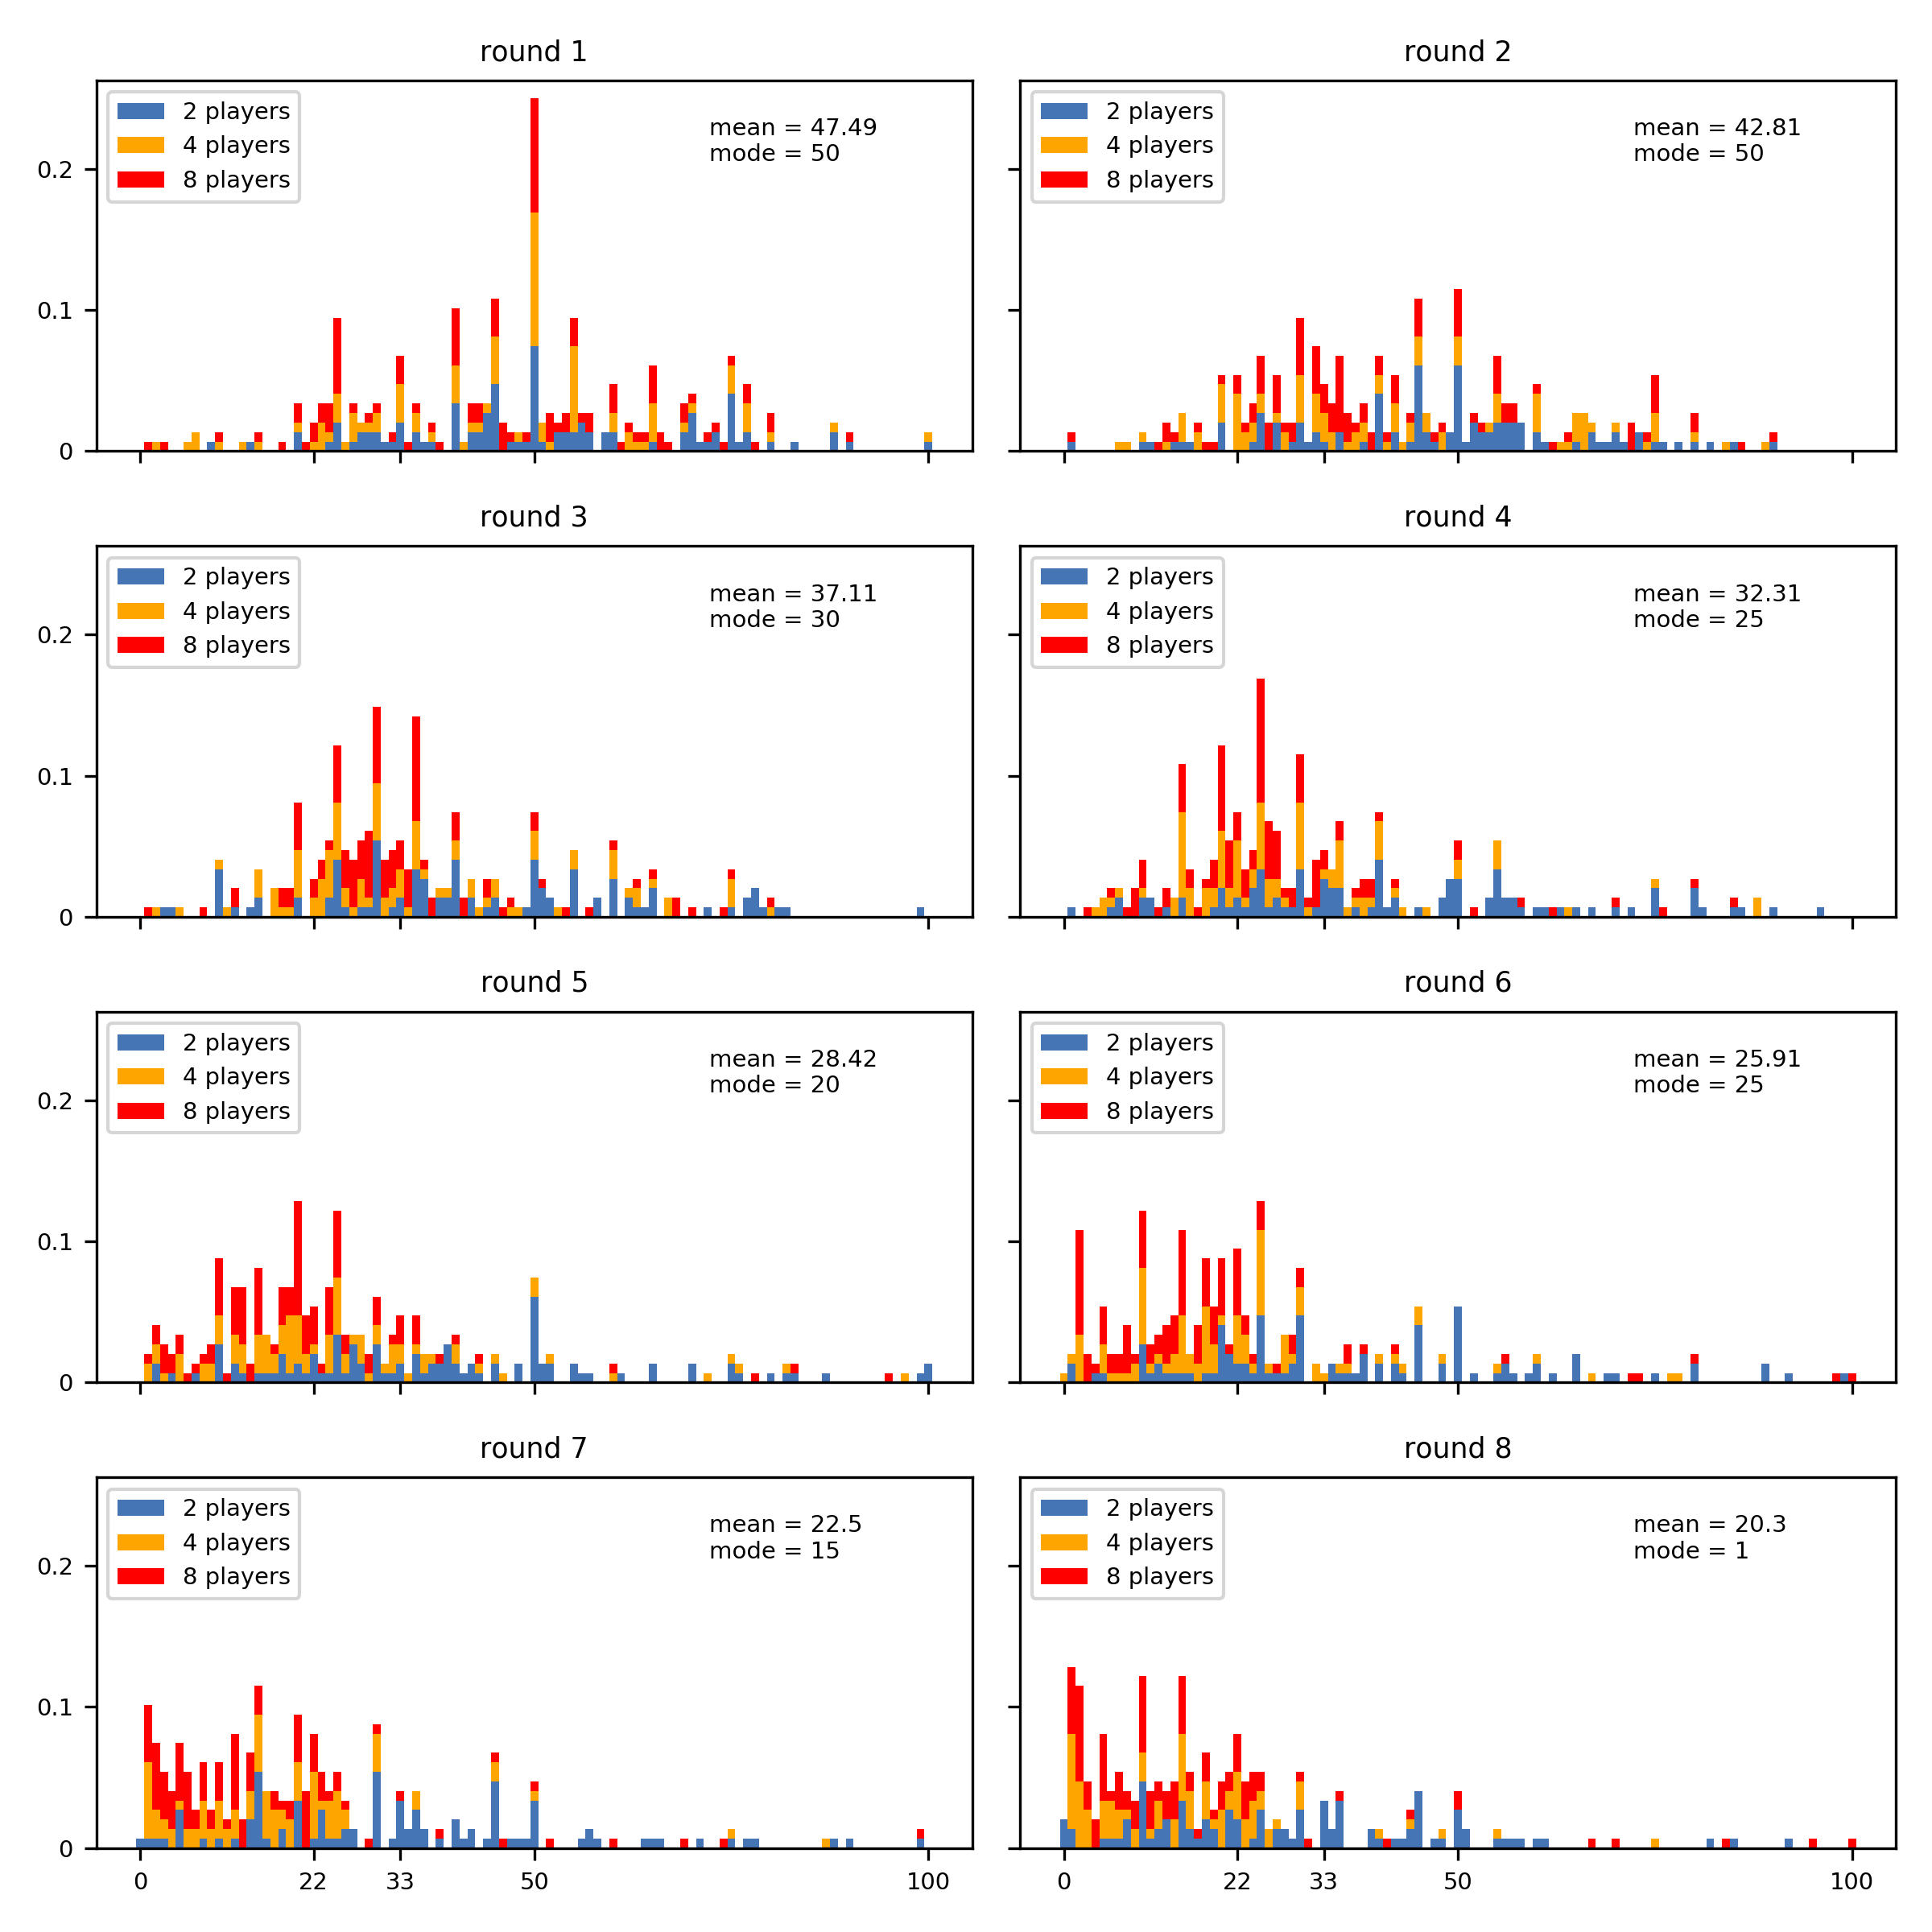
\includegraphics[width=1\textwidth]{../plots/figA5.pdf}\caption{Histograms of guess distributions partitioned into groups and rounds.}
\label{Fig S5}
\end{figure}

Figure \ref{Fig S5} shows the guesses for all eight rounds, partitioned into their respective groups. As can be seen from the histograms, guesses move slowly towards lower numbers in subsequent rounds, with the 2-players groups (in blue) lacking slightly behind the other groups.

\section{Guess Dynamics}
As noted in figure 4 in the main text, players often choose numbers greater than 2/3 of the mean of the previous round. Less than 2\% of all players on AMT never go above 2/3 of the previous mean, while 53\% go above this target more than four times. 

%Figure \ref{Fig S6} shows some examples of the up and down movements of individual guesses from one round to the next. It is difficult to interpret this behavior observed in Fig. S6 as simple directional learning. Instead, players seem to try to “talk” with each other with occasional high guesses, and instead of adapting to the new target (explicitly shown as 2/3 of the previous mean), they may adapt to what they think the other players will guess in the next round.
%
%\begin{figure}
%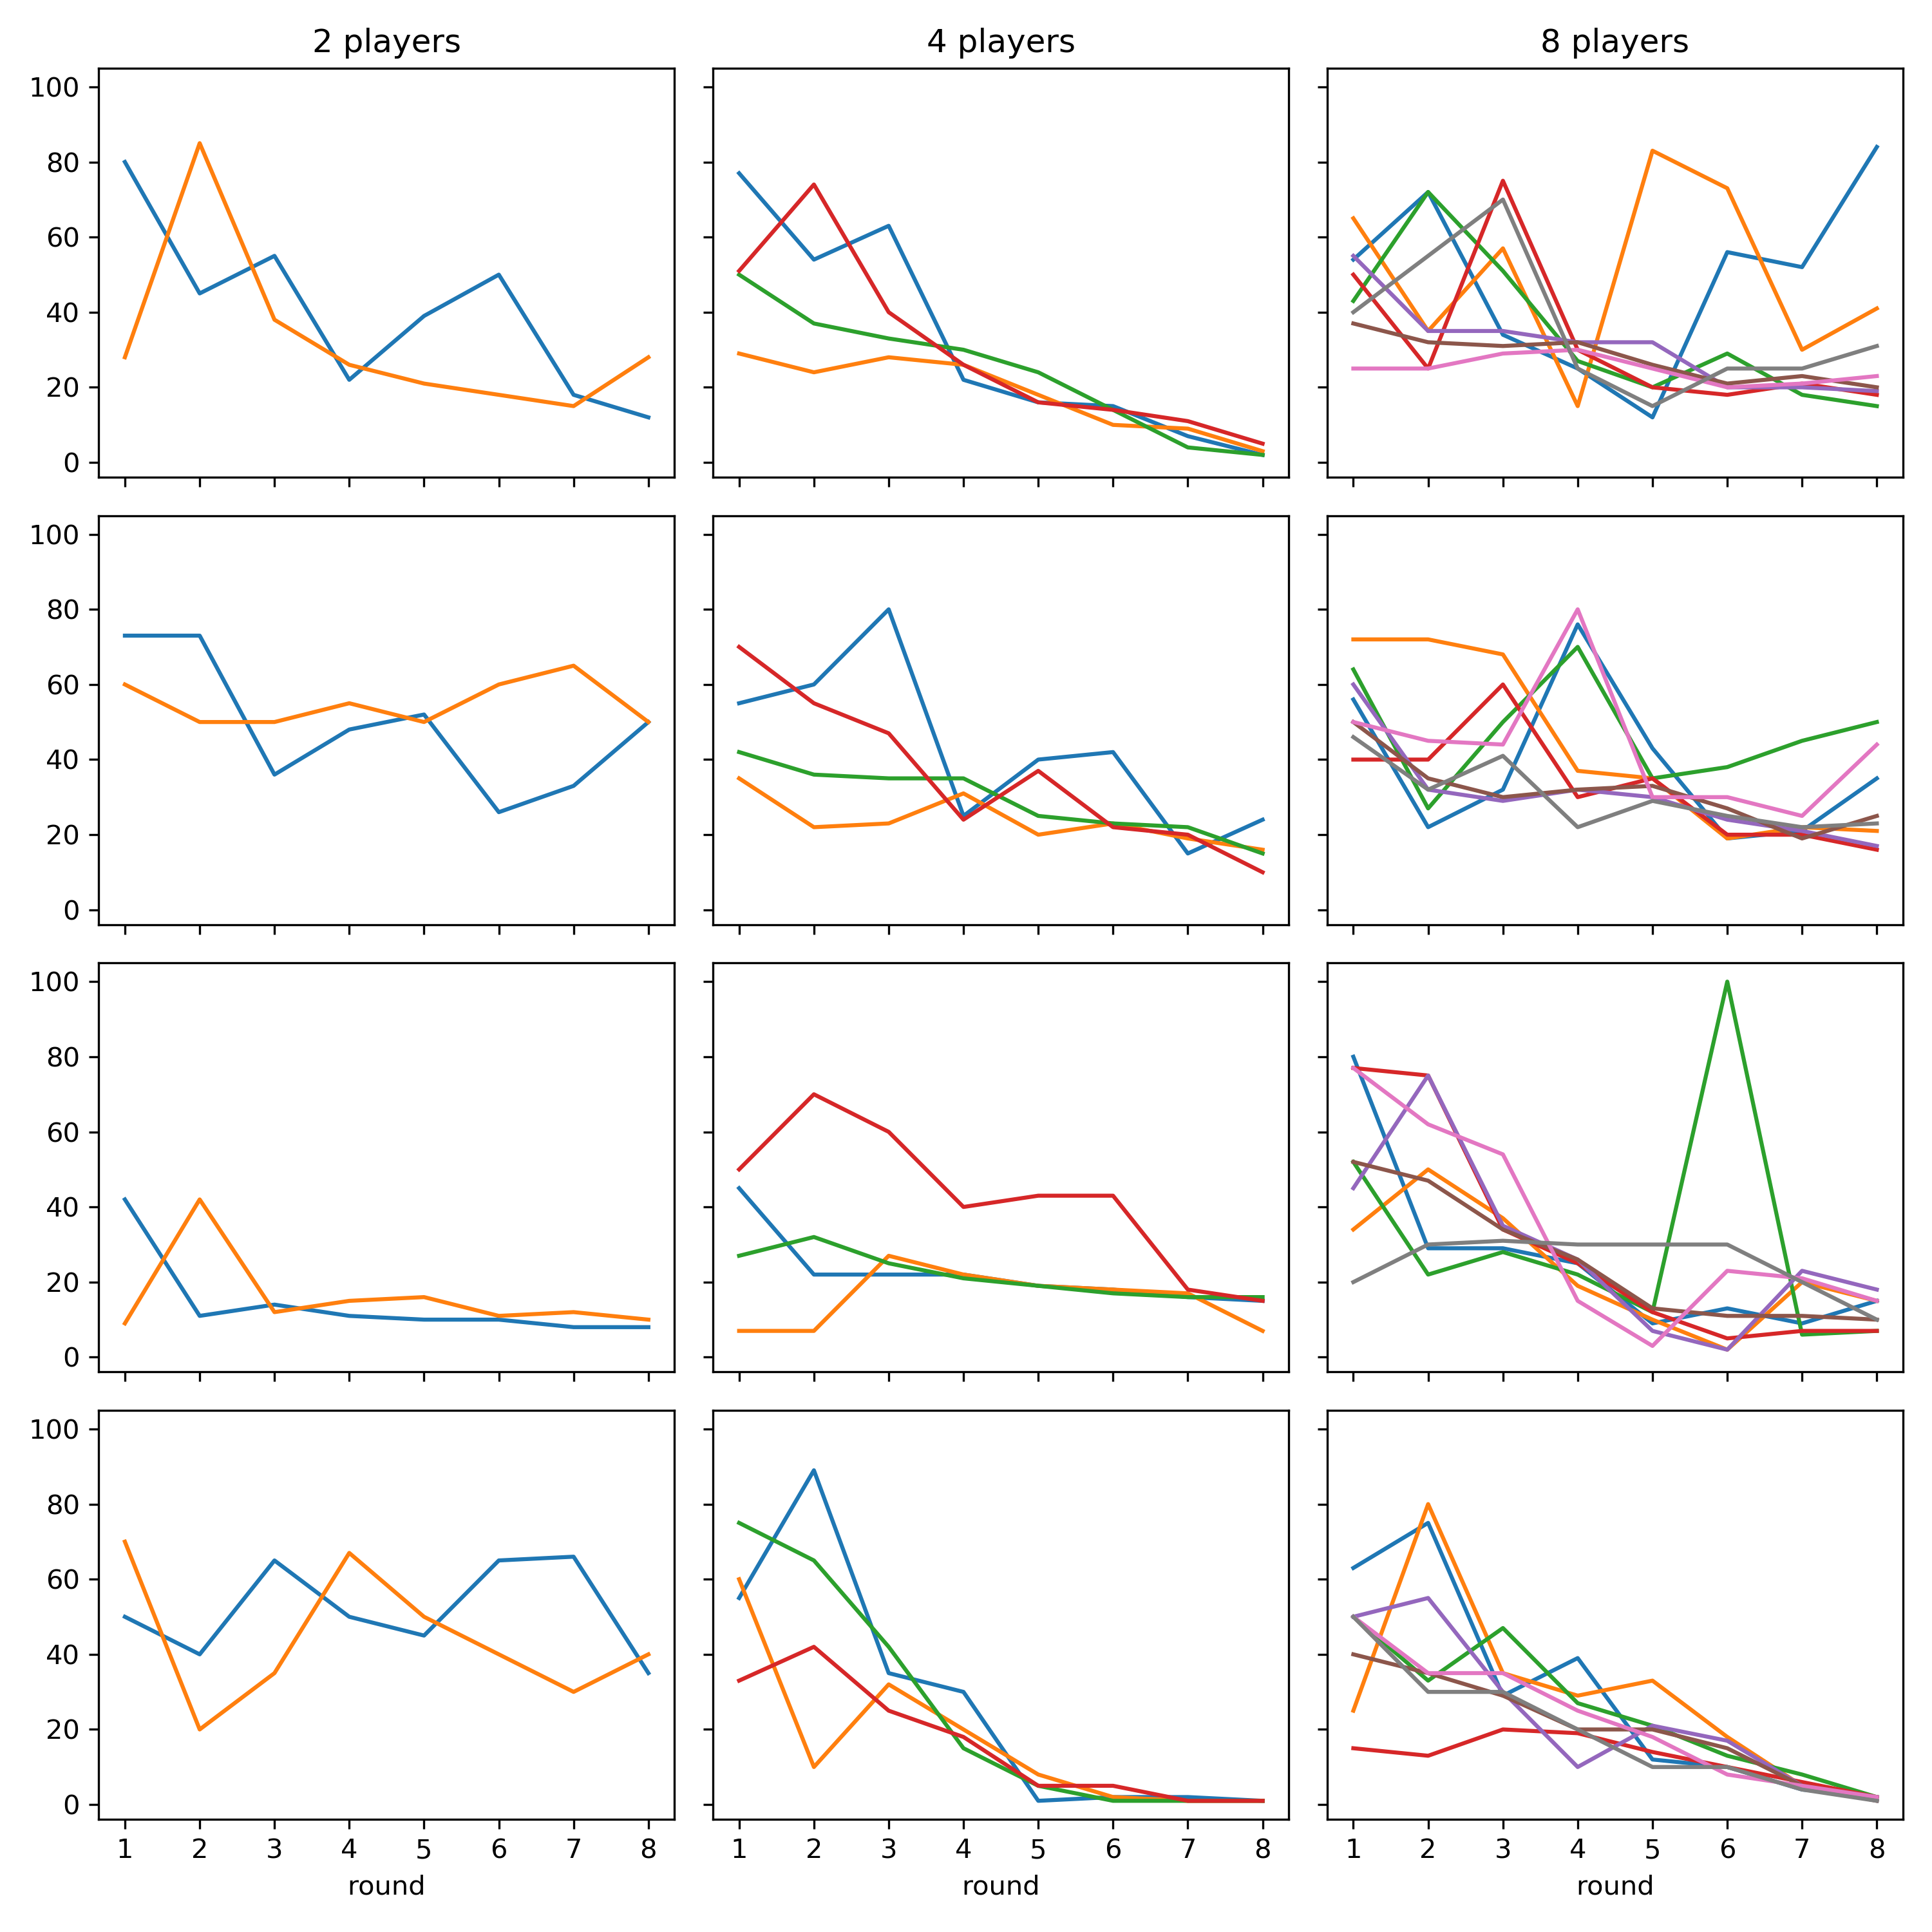
\includegraphics[width=1\textwidth]{../plots/figA6.pdf}\caption{Guess dynamics of player guesses from randomly selected groups.}
%\label{Fig S6}
%\end{figure}
%
%We can illustrate the guess-dynamics in another way as well. 
Figure \ref{Fig S7} shows the dynamics of guesses round by round in such a way that the previous round n is always shown on the x-axis and the next round $n+1$ is always shown on the y-axis. The diagonal black line corresponds to staying at the same guess in subsequent rounds. Lines connecting the dots in Figure \ref{Fig S7} then indicate the sequence of guesses by the same player, whose comments are shown in the legend. The total bonus earned is shown in parenthesis.

\begin{figure}
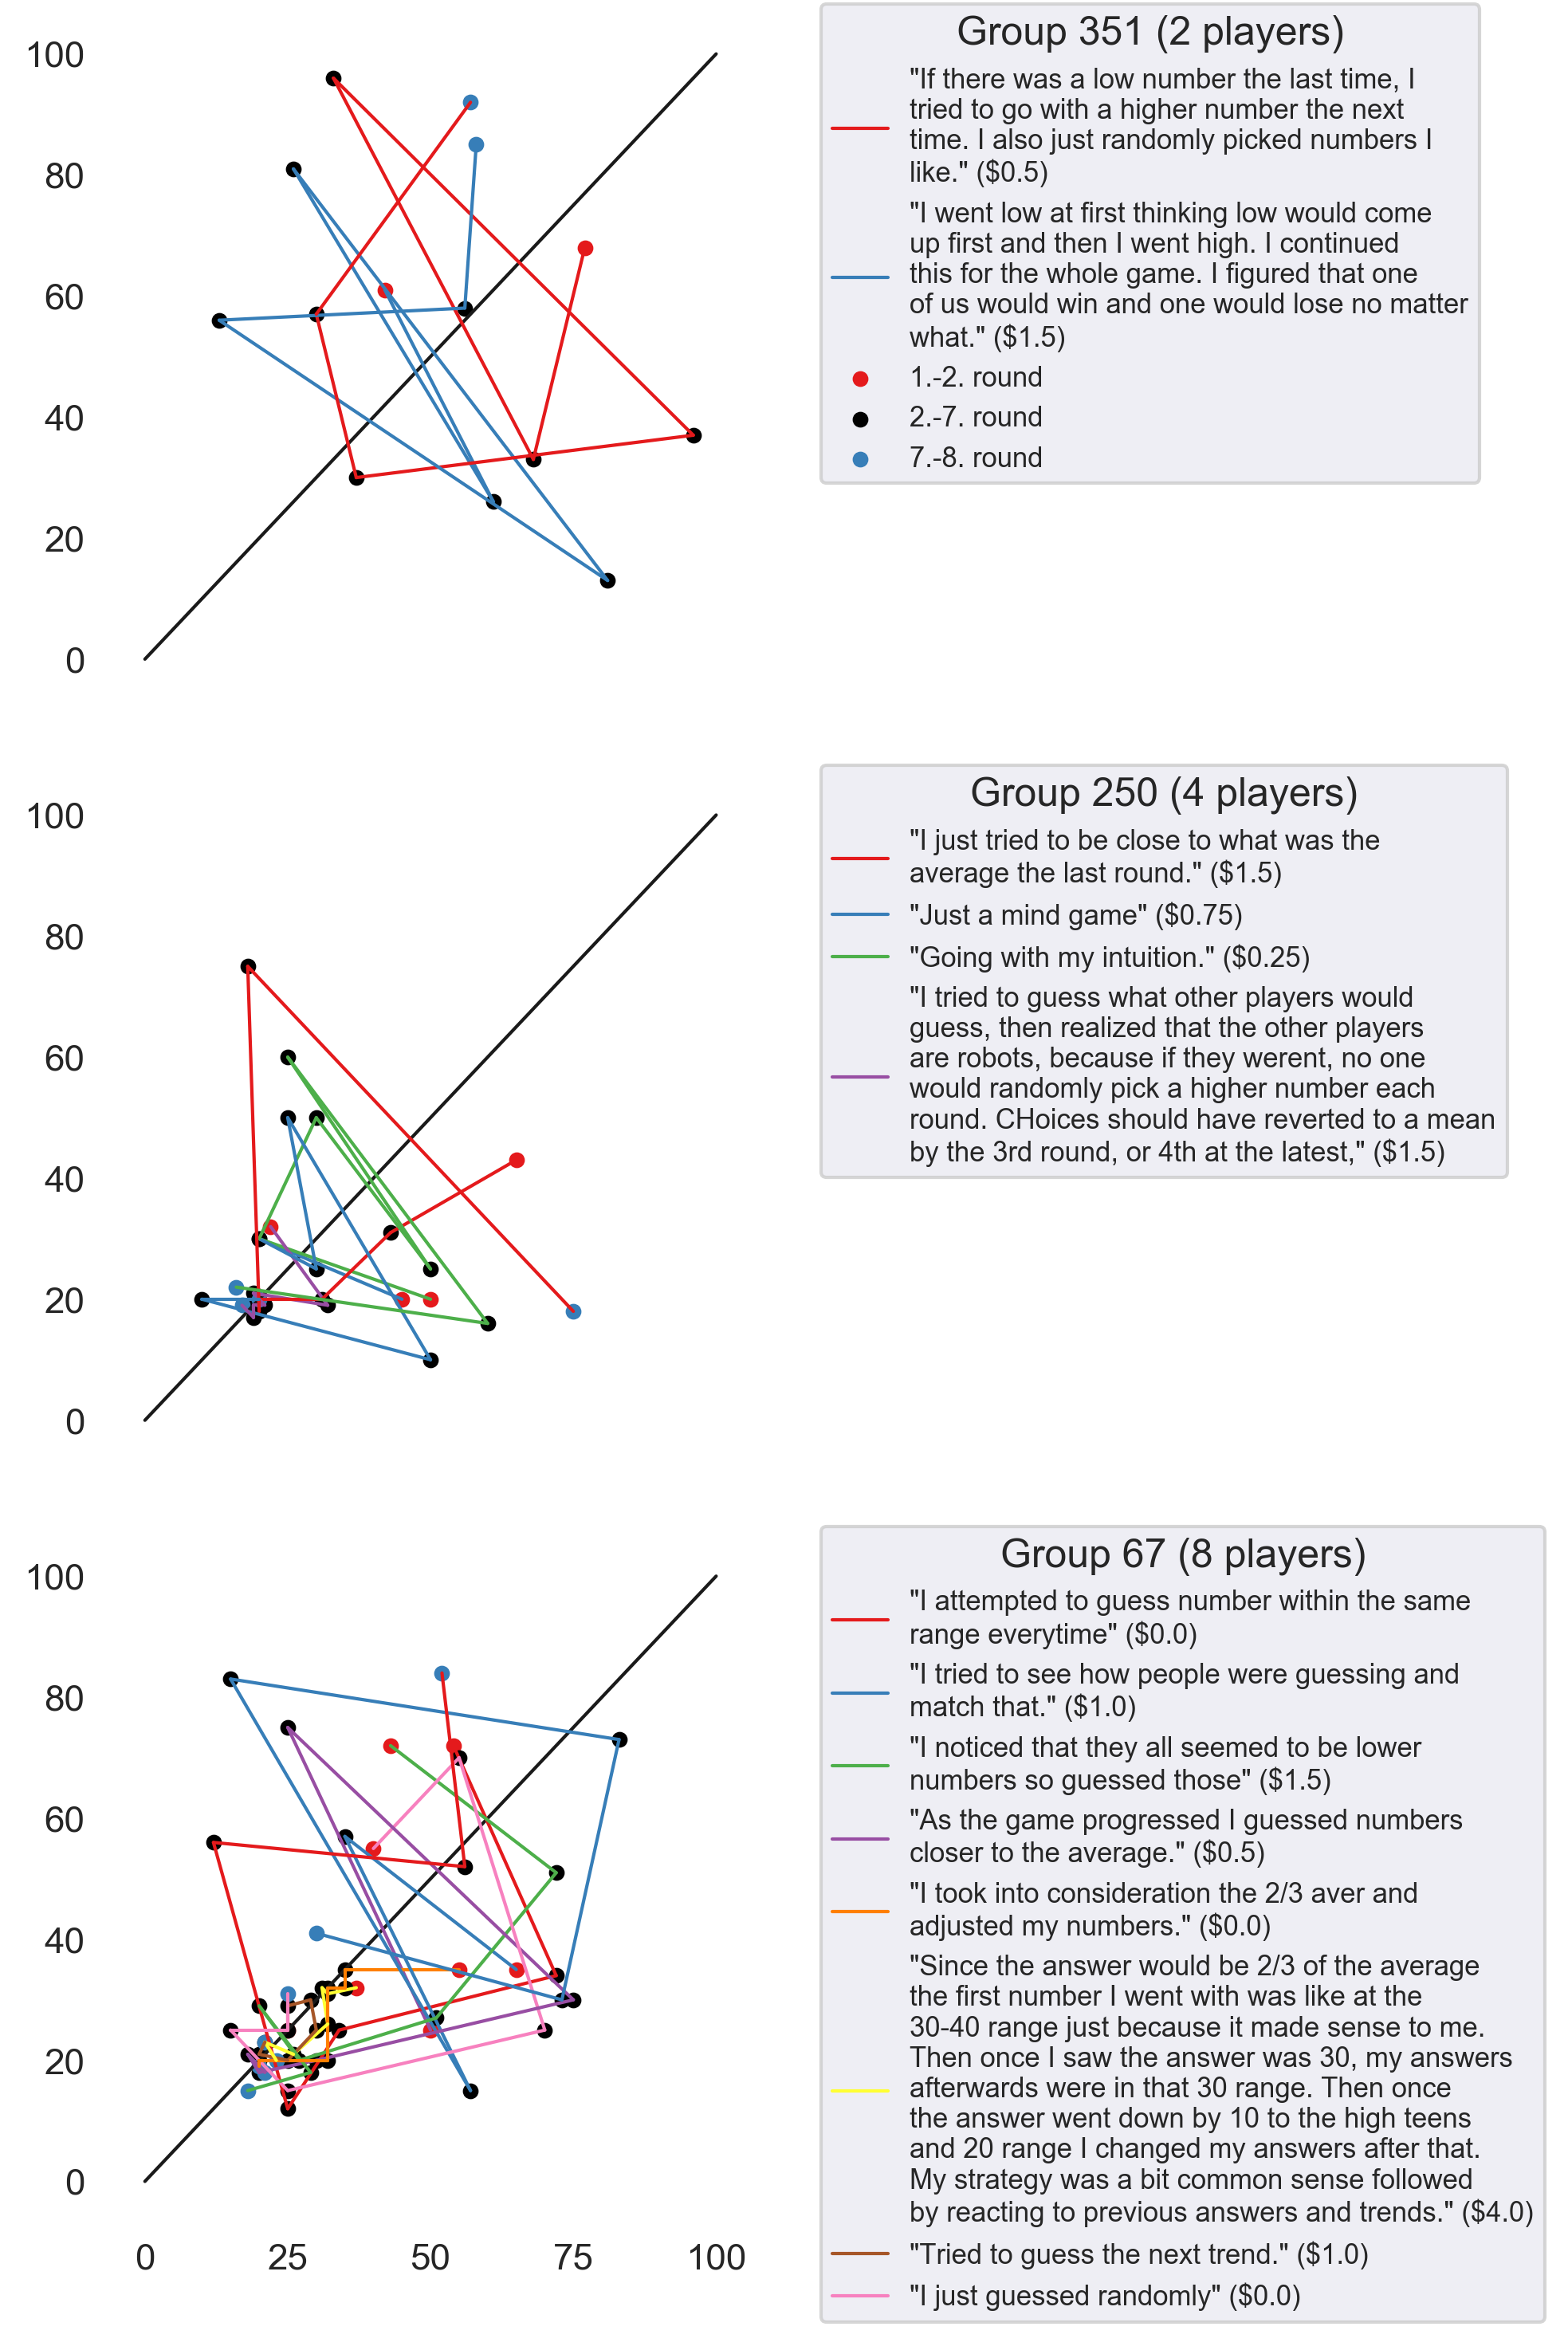
\includegraphics[width=1\textwidth]{../plots/figA7.pdf}\caption{Dynamics of guesses round by round.}
\label{Fig S7}
\end{figure}
